\section*{Дорожная библиотека}
\addcontentsline{toc}{section}{Дорожная библиотека}
\subsection*{Перекрёсток}
\addcontentsline{toc}{subsection}{Перекрёсток}

\textbf{Задание:}\\
Реализовать модель движения транспорта по перекрёстку с применением дорожной библиотеки.\\

\textbf{Решение:}\\
Таким образом, была реализована модель движения транспортных средств по перекрестку, позволившая ознакомиться с основными инструментами дорожной библиотеки среды AnyLogic.Для начала необходимо разметить дорогу, по которой будет передвигаться транспорт, а также дополним карту парковками и автобусными остановками. (Рисунок \ref{fig:basic_traffic1})
\begin{figure}[h]
	\centering 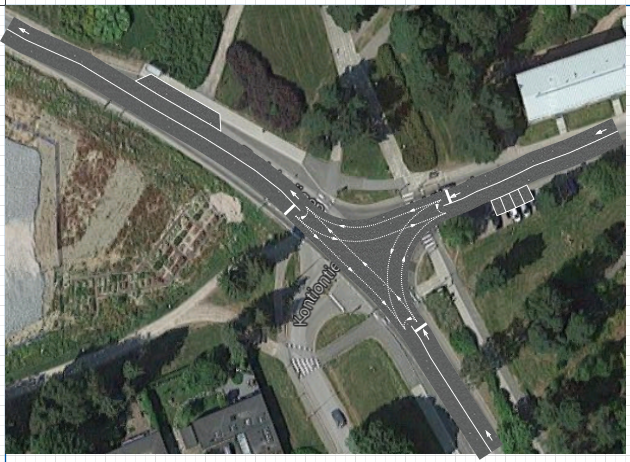
\includegraphics[scale=0.6]{basic_traffic1}
	\caption{Разметка основных объектов дороги}
	\label{fig:basic_traffic1}
\end{figure}

\newpage

Логику модели можно представить с помощью специальных блоков Дорожной библиотеки. (Рисунок \ref{fig:basic_traffic2})
\begin{figure}[h]
	\centering 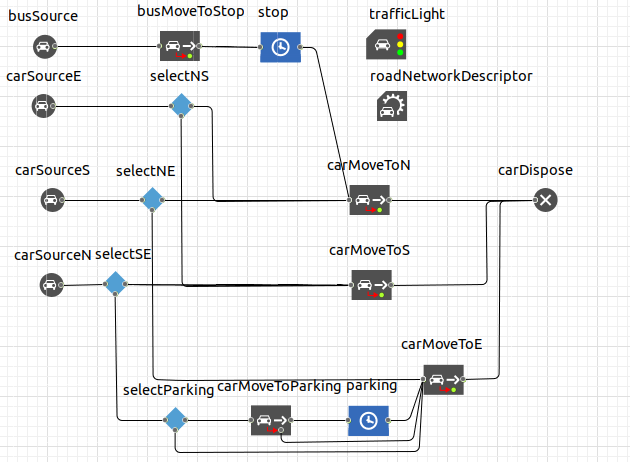
\includegraphics[scale=0.6]{basic_traffic2}
	\caption{Логика дорожных объектов}
	\label{fig:basic_traffic2}
\end{figure}

Имеется три источника машин для трёх разных направлений дороги и один источник автобусов. Если машина едет с севера, то она может поехать в том направлении движения, по которому едет сейчас, может поехать на восток, может поехать на парковку если имеются свободные места.\\

При выборе движения прямо или на восток в конце дороги машины выходят из модели, в случае если было решено припарковать машину, она при помощи блока \textit{Delay} задержится на парковке некоторое время, после чего вновь поедет на восток.\\

Для машин, едущих с юга имеется несколько вариантов движения. Они могут поехать на север или поехать на восток.\\

Если машина едет с востока, то она может поехать на север или на юг.\\

Автобусы движутся к остановке, где стоят некоторое время после чего продолжают свое движение на север.\\

Также были установлены светофоры на главном перекрёстке и блоки, отображающие плотность загруженности участков дороги. (Рисунок \ref{fig:basic_traffic3})

\begin{figure}[h]
	\centering 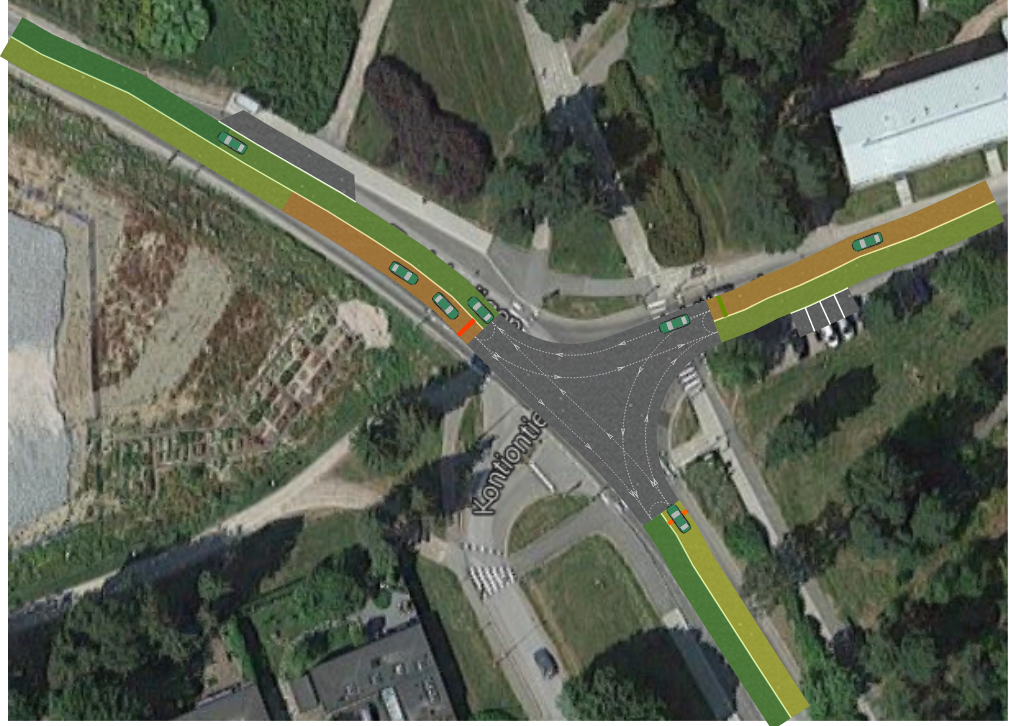
\includegraphics[scale=0.35]{basic_traffic3}
	\caption{Работа модели в 2D}
	\label{fig:basic_traffic3}
\end{figure}

\begin{figure}[h]
	\centering 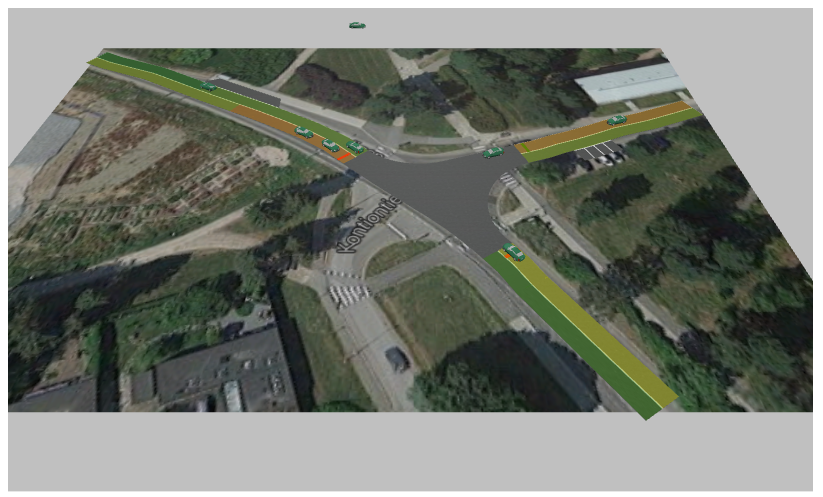
\includegraphics[scale=0.35]{basic_traffic4}
	\caption{Работа модели в 3D}
	\label{fig:basic_traffic4}
\end{figure}

Таким образом, была реализована модель движения транспортных средств по перекрестку.